\chapter{Introduction}

\section{Background}
\textbf{Ghana characteristics}
Ghana’s northern part climate is labelled as semi-arid savannah-like. High temperatures are common and on a yearly basis the short rainy season is out-performed by long periods of drought. As a source of water supply, groundwater is abstracted from its surroundings. The relatively high-quality water is collected and mainly used for domestic purposes, livestock and construction. In more restricted quantities groundwater is used for irrigation. The use of groundwater prevents farmers from incurring potential losses in crop production and increases yields. \bigskip\\
For as long as natural recharge rates exceed discharge, the used groundwater is renewable and the water source is stated to be sustainable. It is roughly estimated the environment has the capability to naturally recharge a maximum of 2.5-10\% of the annual rainfall. Based on the rainfall data for northern Ghana this results in an estimated long term annual natural recharge of 60 mm/y. Currently, local groundwater use is estimated to be approximately 5\% of this annual recharge (Martin, 2006). The amount of water withdrawn is marginal and the environment is therefore self-reliant. However, fluctuations in groundwater use over time and place do occur. Accurate field data on these fluctuations is lacking. Recent observations show wells drying out and groundwater tables falling, both indicators of possible unsustainable groundwater use.
\bigskip\\
Following the trend seen in previous decades, it is expected future groundwater production will further increase. An overall improvement of the Ghanaian energy network as well as lower energy costs will make groundwater more accessible via electrical pumps. In general, this will lead to more extensive use of groundwater in the ongoing battle against shortages in clean drinking water. On top of this the national government aims at becoming more self-sufficient. Policies are pointed at more intensive agricultural development in the northern regions of Ghana (Wood, 2013). Optimization in field irrigation has the potential to increase yields and even double the number of crops produced per year (Owusu et al., 2017). Consequently, the need for groundwater abstraction becomes substantially higher. Climate change can potentially have a negative influence on the natural recharge. While the need will be higher, natural recharge volumes can become lower. In the near future it is possible that discharge rates will exceed natural recharge and the abstracting of groundwater is no longer sustainable. Objective of this research is to explore the possibilities of scaling up artificially managed aquifer recharge (MAR) for aquifer storage and recovery (ASR) to contribute towards the continued sustainable use of groundwater in the northern regions of Ghana. 

\section{Research gap}
\textbf{ASR systems}


blabla
\begin{figure}[h!]
	\centering
	\begin{subfigure}[b]{0.5\linewidth}
		\centering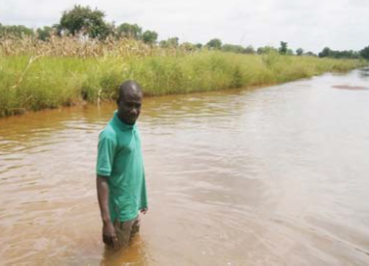
\includegraphics[width=0.8\linewidth]{Flood}
		\captionsetup{justification=centering}		
		\caption{\label{fig:Flood}}
		\end{subfigure}%\hfill
	\begin{subfigure}[b]{0.5\linewidth}
        \centering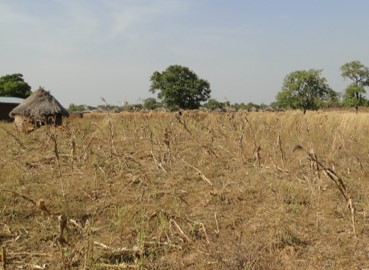
\includegraphics[width=0.8\linewidth]{Drought}
		\captionsetup{justification=centering}		
		\caption{\label{fig:Drought}}
		\end{subfigure}
		\captionsetup{justification=centering}	
	\caption[Example on (\subref{fig:Flood}) flood near Weisi, Upper West Region and (\subref{fig:Drought}) drought near Nungo, Upper East Region]{Example on (\subref{fig:Flood}) flood near Weisi, Upper West Region (source: Owusu et al., 2017) and (\subref{fig:Drought}) drought near Nungo, Upper East Region} 
	\label{fig:Flood_Drought}
\end{figure} \\

\begin{figure}[h]
 \centering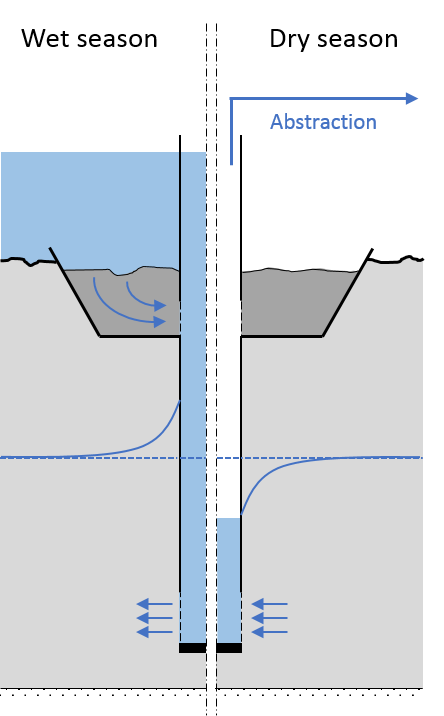
\includegraphics[width=0.4\linewidth]{Wet_Dry}
 \captionsetup{justification=centering}
 \caption{Principle Aquifer Storage \& Recovery (ASR) system}
 \label{fig:ASR}
\end{figure}

\section{Research purpose}\

\textbf{PIT \& Irrigation purpose}
PIT application on irrigation (single figure). and the desired upscaling of this system (multiple figure). 

\begin{figure}[h]
 \centering
\includegraphics[width=0.8\linewidth]{Purpose}
 \captionsetup{justification=centering}
 \caption[Schematic: dry season system use]{Schematic: dry season system use \\ (visual support by Housin Aziz, Jhun Capaya and Nibras@design from Noun Project - \url{https://thenounproject.com})}
 \label{fig:Purpose}
\end{figure}

\begin{figure}[h]
 \centering
\includegraphics[width=0.8\linewidth]{Purpose_Multi}
 \captionsetup{justification=centering}
 \caption[Schematic: desired up-scaling in dry season system use]{Schematic: desired up-scaling in dry season system use \\ (visual support by Housin Aziz, Jhun Capaya and Nibras@design from Noun Project - \url{https://thenounproject.com})}
 \label{fig:Purpose_Multi}
\end{figure}

resulting in a research question

\textbf{Research question}\

How can scaled-up Aquifer Storage and Recovery (ASR) systems be beneficial for the availability and sustainable use of agricultural groundwater in northern Ghana? \\

How can scaled-up Aquifer Storage and Recovery (ASR) systems be beneficial for the availability and sustainable use of groundwater in northern Ghana agriculture?

\section{Reader's guide}\
to answer this research question... 
